% INTRODUÇÃO-------------------------------------------------------------------

\chapter{INTRODUÇÃO}
\label{chap:introducao}

Alguns programas podem ser utilizados para auxílio da escrita do TCC entre eles o \textit{MathType} (com relação a equações), \textit{Inkscape} (com relação a imagens). \\ %enter

\textbf{PRIMEIRAS ORIENTAÇÕES}\\ %\textbf - negrito

1) O comando ``$\backslash$autoref\{label\}'' auto referencia o respectivo ``\textit{label}".

Exemplo 1: De acordo com o exposto no \autoref{chap:introducao}... Pode-se verificar na \autoref{fig:consumomundialporfonte-fig1}...\\

2) O comando ``$\backslash$citeonline\{bibid\}'' é utilizado para citações diretas. Ele cita o respectivo ``\textit{bibid}".\\

Exemplo 2:  Conforme \citeonline{AMARANTEMESQUITA20141261} cita em seu artigo, turbinas hidrocinéticas atualmente têm... \citeonline{VAZ2018509} também ressalta que turbinas de eixo horizontal possuem maiores...\\

\citeonline{vallverdu2014}  --->  Vallverdú (2014) --- DIRETA

\cite{vallverdu2014}   --->  (VALLVERDÚ, 2014) --- INDIRETA\\

O comando ``$\backslash$cite\{bibid\}'' é utilizado para citações indiretas. Ele cita o respectivo ``\textit{bibid}".\\

Exemplo 3: A máxima eficiência que uma turbina hidrocinética ideal pode alcançar é dada pelo Limite de Betz-Joukowski que corresponde a 59,3\%, o equivalente a um $C_P$ de 0,593 \cite{vallverdu2014, SHINOMIYA2015d}.\\ %Ao colocar a virgula, pode-se adicionar mais de um autor à citação.

3) Um ponto final é representado por um espaço entre os parágrafos.

Exemplo 1.
Exemplo 2.

Exemplo 3.

Exemplo 4.\\

4) Figuras

Figuras com extensão .jpg, .pdf, .eps, .ps, .png

As figuras devem ser adicionadas a pasta ``$\backslash$figuras'' no diretório deste template.

%[!htb] - são as opções onde o LaTeX escolhe a melhor posição para inserir a figura na página, aqui (here), topo (top) ou embaixo (bottom), respectivamente. Se você colocar apenas um deles, por exemplo [!h], a figura ficará exatamente onde você inseriu.

%Modelo de inclusão de figura. É só copiar, tomar como modelo e modificar.
\begin{figure}[H]
	\centering
	\caption{Consumo mundial de energia por fonte de energia em quatrilhões de BTU.}
	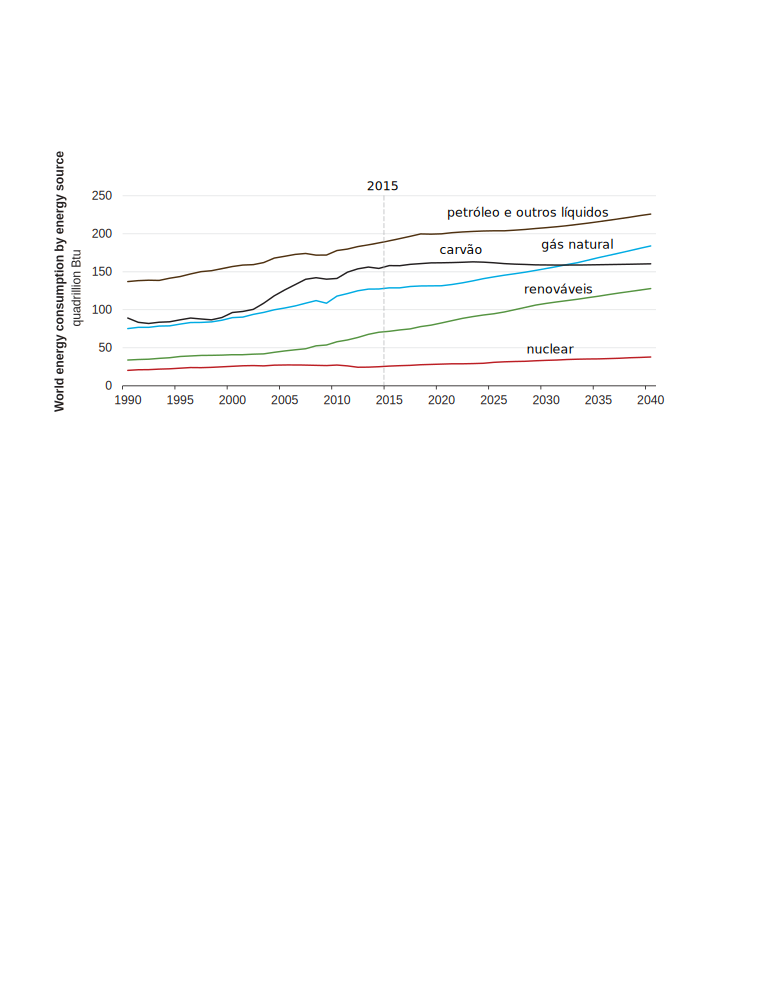
\includegraphics[width=1.0\textwidth]{figuras/consumodeenergiamundialporfonte.pdf}
	\fonte{\citeonline{harris2006essential}.}
	\label{fig:consumomundialporfonte-fig1}
\end{figure}

5) Referências

As referências devem ser adicionadas no arquivo ``base-referencias.bib'' no diretório deste template. 

Modelos podem ser editados na página ``https://truben.no/latex/bibtex/''. A partir do DOI pode-se encontrar o arquivo \textit{.bib} em ``https://www.doi2bib.org/''. No Google Acadêmico também se encontram bastantes referências no formato \textit{.bib}.

Tome cuidado com autores com nomes que termiam em Júnior, Filho, Neto e etc. Forma correta: ``Fulano Deltrano Siclano\{ \}Neto''.

As referências não reconhecem legal os pacotes de acentos. Então deve-se utilizar comandos de acentos. ``http://latexbr.blogspot.com/2011/02/acentos-e-caracteres-especiais.html''.

*Ao ser executado pela primeira vez, possa ser que você precise está conectado a internet para o programa instalar os \textit{packages} necessários para compilar o arquivo PDF.

Utilize esse \textit{template} sempre verificando as normas da Biblioteca Central da UFPA segundo o Guia para Elaboração de Trabalhos Acadêmicos disponível em http://bc.ufpa.br/ além das normas da ABNT.

Outras orientações podem ser encontradas na internet.\\

Boa escrita!

\section{Objetivos}
\label{sec:objetivos}

\subsection{Objetivo geral}
\label{subsec:objetivogeral}

Escreva seu objetivo geral aqui.

\subsection{Objetivos específicos}
\label{subsec:objetivosespecificos}

\begin{itemize}
\item Escreva seu objetivo específico 1 aqui;
\item Escreva seu objetivo específico 2 aqui;
\item ...;
\end{itemize}

\section{Estrutura do trabalho}
\label{sec:estrututaTrabalho}

Este trabalho está dividido em cinco seções, referências, anexos e apêndices.

Na seção 1 é apresentado o contexto no qual o trabalho está inserido, a justificativa e os objetivos almejados...

A revisão bibliográfica sobre as temáticas relacionadas com essa pesquisa é apresentada na seção 2...

A seção 3 mostra conceitos teóricos relacionados às ferramentas utilizadas no estudo tal como...

Na seção 4, os resultados são apresentados juntamente com suas devidas discussões, verificando...

Finalizando, a seção 5 faz as devidas conclusões e apresenta sugestões para trabalhos futuros.
